\documentclass[pdftex,12pt]{beamer}
\usepackage[italian]{babel}
%~ \usepackage[latin1]{inputenc}
\usepackage[utf8]{inputenc}


%inclusione immagini:
\usepackage{graphicx}
%~ \usepackage{multicol}

%inclusione codice:
%~ \usepackage{listings}

\usepackage{amsmath}
\usepackage{amssymb}
\usepackage{amsfonts} 
\usepackage{multicol}
\usepackage{xcolor}
\usepackage{listings}
\usepackage{algorithm}
\usepackage{algorithmic}
\usepackage{array}
\usepackage{multirow}
\usepackage{booktabs}
\usepackage{url}
\usepackage{textcomp}


%~ \usepackage[dvips]{graphicx}
%\graphicspath{{figures/}}

%~ NON SI POSSONO INSERIRE IMMAGINI IN EPS!
\DeclareGraphicsExtensions{.png, .jpg, .jpeg, .pdf}
%~ \usepackage[pdftex]{graphicx}

\usepackage{acronym}
\colorlet{newred}{red!60!black}
\setbeamercolor{block title}{bg=newred,fg=white}%bg=background, fg= foreground
\setbeamercolor{block body}{bg=white,fg=black}%bg=background, fg= foreground
\setbeamercolor{frametitle}{fg=newred}

\newcommand{\textCl}[1]{\textcolor{blue}{#1}}
%\usecolortheme{whale}	
\usetheme{CambridgeUS}
\usepackage{textcomp}
\definecolor{listinggray}{gray}{0.9}
\definecolor{lbcolor}{rgb}{0.9,0.9,0.9}
\lstset{
	language=Java,                % the language of the code
	basicstyle=\small\footnotesize,           % the size of the fonts that are used for the code
	numbers=left,                   % where to put the line-numbers
	numberstyle=\tiny\color{gray},  % the style that is used for the line-numbers
	stepnumber=1,                   % the step between two line-numbers. If it's 1, each line 
                                  % will be numbered
	numbersep=5pt,                  % how far the line-numbers are from the code
	backgroundcolor=\color{white},      % choose the background color. You must add \usepackage{color}
	showspaces=false,               % show spaces adding particular underscores
	showstringspaces=false,         % underline spaces within strings
	showtabs=false,                 % show tabs within strings adding particular underscores
	frame=single,                   % adds a frame around the code
	rulecolor=\color{black},        % if not set, the frame-color may be changed on line-breaks within not-black text (e.g. commens (green here))
	tabsize=2,                      % sets default tabsize to 2 spaces
	captionpos=b,                   % sets the caption-position to bottom
	breaklines=true,                % sets automatic line breaking
	breakatwhitespace=false,        % sets if automatic breaks should only happen at whitespace
	title=\lstname,                   % show the filename of files included with \lstinputlisting;
                                  % also try caption instead of title
	keywordstyle=\color{blue},          % keyword style
	commentstyle=\color{green},       % comment style
	stringstyle=\color{magenta},         % string literal style
	escapeinside={\%*}{*)},            % if you want to add a comment within your code
	%  morekeywords={*,...}               % if you want to add more keywords to the set
}
\title[Java]{
Corso di base di JAVA
}

\author[Mauro Donadeo]{
	mauro.donadeo@gmail.com
}

\institute[HTLAB]{
	Università degli Studi di Padova
}
\logo{
\includegraphics[width=5mm]{images/logo.png}}
\date[05.04.2012]{5 aprile 2012}

\setbeamertemplate{navigation symbols}{}
\begin{document}
\begin{frame}
	\setbeamercolor{block body}{bg = yellow}
	\begin{block}{}
		\begin{center}
			{\large\textbf{Corso di base JAVA}}\\
			\itshape{Mauro Donadeo}\\
			mail: mauro.donadeo@gmail.com
		\end{center}
	\end{block}
	\setbeamercolor{block body}{bg = white}
	\begin{block}{}	
		\begin{center}
			\begin{huge}
			Iterazioni
			\end{huge}\\
			
\includegraphics[width = 30mm]{images/java-logo.jpg}
		\end{center}
	\end{block}	
\end{frame}

\section*{Complementi}
\subsection*{Switch}
\begin{frame}[fragile]
\frametitle{Complementi}
\begin{block}{Enunciato switch}
Una sequenza di confronti in un'\textbf{unica variabile intera} con diverse \textbf{alternative costanti} può essere realizzata con 
l'enunciato \alert{switch}
\end{block}
\begin{columns}
\begin{column}{0.4\textwidth}
\begin{lstlisting}
int x;
int y;
...
if (x == 1)
   y = 1;
else if (x == 2)
   y = 4;
else if (x == 4)
   y = 16;
else
   y = 0;
\end{lstlisting}
\end{column}
\begin{column}{0.55\textwidth}
\begin{lstlisting}
int x;
int y;
...
switch (x){ 
    case 1: y = 1; break;
    case 2: y = 4; break;
    case 4: y = 16; break;
    default: y = 0; break;
}
\end{lstlisting}
\end{column}
\end{columns}
\end{frame}

\begin{frame}
\begin{block}{L'enunciato switch}
\begin{itemize}
\item \textbf{Vantaggio:} non bisogna ripetere il nome della variabile;
\item \textbf{Svantaggio:}
\begin{itemize}
\item non si può usare se la variabile da confrontare non è intera
\item Non si può usare se uno dei valori da confrontare non è costante
\item in ogni \textbf{\texttt{case}} deve terminare con un enunciato \textbf{\texttt{break}}, altrimenti viene eseguito anche il corpo
del \textbf{\texttt{case}} successivo. \textit{Fonte di molti errori}
\end{itemize}
\end{itemize}
\end{block}
\end{frame}

\subsection*{Operatori relazionali}
\begin{frame}
\frametitle{Errori con gli operatori relazionali}
\begin{block}{}
Alcune espressioni ``naturali'' con operatori relazionali sono errate, ma per fortuna il compilatore le rifiuta
\begin{itemize}
\item \textbf{if(0 \alert{$<=$} x \alert{$<=$} 1)} \textbf{\alert{NON FUNZIONA}}.
\item \textbf{if(0 $<=$ x $\&\&$ x $<=$ 1)} \textbf{OK}
\item \textbf{if(x \alert{$\&\&$} y $>$ 0)} \textbf{\alert{NON FUNZIONA}}
\item \textbf{if(x $>$ 0 \alert{$\&\&$} y $>$ 0)} \textbf{OK}
\end{itemize}
\end{block}
\end{frame}

\begin{frame}
\frametitle{ESERCITAZIONE}
\begin{block}{}
Si scriva la classe \textbf{Triangolo} che descrive un triangolo, la cui interfaccia pubblica vi verrà mostrata tra poco. Collaudare
la classe \textbf{Triangolo} con la classe di prova \textbf{TriangoloTester}, che legge i dati da standard input.
\end{block}
\end{frame}
\section*{Iterazioni}
\subsection*{Ciclo WHILE}
\begin{frame}
\begin{block}{Problema}
Riprendiamo un problema visto nella prima lezione, per il quale abbiamo individuato un algoritmo senza realizzarlo:
\begin{itemize}
\item \textbf{Problema:} Avendo depositato ventimila euro in un conto bancario che produce il 5\% di interessi all'anno, capitalizzati 
annualmente, quanti anni occorrono affinché il saldo del conto arrivi al doppio della cifra iniziale?
\item Abbiamo bisogno di un programma che ripeta degli enunciati (capitalizzazione degli interessi annuali, incremento del conto degli 
anni), finché non si realizza la condizione desiderata
\end{itemize}	
\end{block}
\end{frame}

\begin{frame}
\begin{block}{Enunciato while}
L'enunciato \textbf{while} consente la realizzazione di programmi che devono eseguire ripetutamente una serie di azioni finché è 
verificata una condizione
\end{block}
\begin{block}{Algoritmo che risolve il problema}
\begin{enumerate}
\item All'anno 0 il saldo è 20000
\item \textbf{\textCl{Ripetere}} i passi 2 e 3 \textbf{\textCl{finché}} il saldo è minore del doppio di 20000, poi passare al punto 4.
\item aggiungere 1 al valore anno corrente;
\item il nuovo saldo è il valore del saldo precedente moltiplicato per 1.05.
\item il risultato è il valore dell'anno corrente.
\end{enumerate}
\end{block}
\end{frame}

\begin{frame}
\begin{columns}
\begin{column}{0.5\textwidth}
\begin{block}{Il ciclo while}
\begin{itemize}
\item Sintassi:
\begin{itemize}
\item \textbf{\textCl{while(\alert{condizione})}}\\
\hspace{0.5cm}\textbf{\alert{enunciato}}
\end{itemize}
\item Scopo:
\begin{itemize}
\item eseguire un enunciato finché la condizione è vera
\end{itemize}
\item Il \textbf{\textCl{corpo}} del ciclo \textbf{while} può essere un enunciato qualsiasi, quindi anche un blocco di enunciati
\item L'enunciato \textbf{while} realizza un \textbf{\alert{ciclo}}
\end{itemize}
\end{block}
\end{column}
\begin{column}{.5\textwidth}
\centering
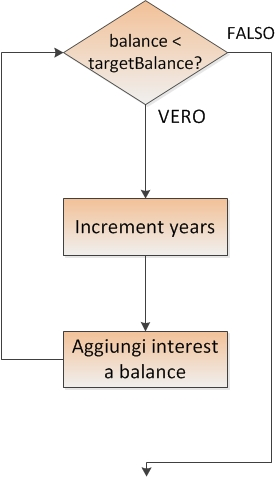
\includegraphics[scale=0.6]{images/CicloWhile.jpg}
\end{column}
\end{columns}
\end{frame}

\begin{frame}[fragile]
\begin{lstlisting}
public class Investment{
    public Investment(double aBalance, double aRate){ 
       balance = aBalance;
       rate = aRate;
       years = 0;
    }
    public void waitForBalance(double targetBalance){ 
        while (balance < targetBalance){ 
            years++;
            double interest = balance * rate / 100;
            balance = balance + interest;
        }
    }
    public double getBalance(){return balance;}
    public int getYears(){return years;}
    private double balance;
    private double rate;
    private int years;
}
\end{lstlisting}
\end{frame}

\begin{frame}[fragile]
\begin{lstlisting}
public class InvestmentTester{
    public static void main(String[] args){
        final double INITIAL_BALANCE = 10000;
        final double RATE = 5;
        Investment invest = new Investment(INITIAL_BALANCE, RATE);
        invest.waitForBalance(2 * INITIAL_BALANCE);
        int years = invest.getYears();
        System.out.println("The investment doubled after "+ years + " years");
    }
}
\end{lstlisting}
\end{frame}

\begin{frame}[fragile]
\frametitle{Cicli infiniti}
\begin{block}{}
Esistono errori logici che impediscono la terminazione di un ciclo, generando un \textbf{\alert{ciclo infinito}}
L'esecuzione del programma continua \textbf{\alert{ininterrottamente}}
\end{block}
\begin{lstlisting}
int year = 0;
while (year < 20){ 
    double interest = balance * rate / 100;
    balance = balance + interest;
}
\end{lstlisting}
\pause
\begin{lstlisting}
int year = 20;
while (year > 0){
    year++;
    double interest = balance * rate / 100;
    balance = balance + interest;
}
\end{lstlisting}
\end{frame}

\subsection*{Ciclo For}
\begin{frame}
\frametitle{Ciclo for}
\begin{block}{For al posto di while}
Molti cicli hanno questa forma:\\
\textbf{\textCl{i} = \alert{inizio;}}\\
\textbf{while(\textCl{i} $<$ \alert{fine})}\\
\textbf{$\{ \alert{enunciati}; \mbox{ } \textCl{i++}$;\}}
\end{block}
\begin{block}{Sostituzione}
\textbf{Per comodità esiste il \textbf{\textCl{ciclo for equivalente}}}\\
\hspace{0.7cm}\textbf{for(\textCl{i} = \alert{inizio}; \textCl{i} $<$ \alert{fine}; i++)}
\end{block}
\begin{block}{}
Non è necessario che l'incremento sia di una sola unità, né che sia positivo, né che sia intero.
\end{block}
\end{frame}

\begin{frame}[fragile]
\begin{block}{}
\textbf{\textCl{for(\alert{inizializzazione}; \alert{condizione}; aggiornamento)}}\\
\hspace{0.7cm} \textbf{\alert{enunciato}}
\end{block}
\begin{block}{Scopo}
Eseguire un'\textbf{\textCl{inizializzazione}}, poi \textbf{\textCl{ripetere}} l'esecuzione di un enunciato ed effettuare un 
\textbf{\textCl{aggiornamento}} finché la \textbf{\textCl{condizione}} è vera;
\end{block}
\begin{block}{Nota}
L'inizializzazione può contenere la definizione di una variabile, che \textbf{\alert{sarà visibile soltanto all'interno del ciclo}}
\end{block}
\begin{lstlisting}
for (int y = 1; y <= 10; y++){
    //corpo
}
//qui y non e' piu' definita.
\end{lstlisting}
\end{frame}

\begin{frame}[fragile]
\frametitle{Il metodo waitYears di Investment}
Vogliamo sapere quale sarà il saldo finale del nostro investimento dopo 20 anni, con il tasso di interesse costante del 5\%.
\begin{lstlisting}
public class Investment{
     ...
     public void waitYears(int n){
         for (int i = 1; i <= n; i++){
             double interest = balance * rate / 100;
             balance = balance + interest;
         }
         years = years +n;
    }
    ...
}
\end{lstlisting}
\end{frame}

\subsection*{Visibilità delle variabili}
\begin{frame}[fragile]
\frametitle{Visibilità delle variabili}
\begin{block}{}
Se il valore finale di una variabile di controllo del ciclo deve essere visibile al di fuori del corpo del ciclo bisogna definirla 
\textbf{\alert{prima}} del ciclo.
\end{block}
\begin{block}{}
Poiché una variabile definita nell'inizializzazione di un ciclo non è più definita dopo il corpo del ciclo, è possibile (e comodo)
usare di nuovo lo \textbf{\textCl{stesso nome in altri cicli}}
\end{block}
\begin{lstlisting}
double b = 0.3;
for (int i = 1; i < 10 && b < c; i++){ 
    //modifica b
}
// qui b e' visibile, mentre i non lo e'
for (int i = 3; i > 0; i--)
    System.out.println(i);
\end{lstlisting}
\end{frame}

\begin{frame}
\frametitle{ESERCIZIO}
\begin{block}{}
Scrivere un programma che prende in ingresso una stringa e la inverte. Ad esempio se prende in ingresso \textbf{CIAO} dovrà stampare a 
video \textbf{OAIC}
\end{block}
\begin{block}{Suggerimento}
Il metodo \texttt{charAt(i)} restituisce il carattere della stringa alla i-esima posizione.
\end{block}
\end{frame}

\section*{Cicli annidati}
\begin{frame}[fragile]
\frametitle{Cicli annidati}
\begin{block}{Problema}
Vogliamo stampare una tabella con i valori delle potenze \textbf{$x^y$}, per ogni valore di \textbf{x} tra 1 e 4 e per ogni valore
di \textbf{y} tra 1 e 5.
\end{block}
\begin{center}
\begin{tabular}{|c c c c c|}
\hline
1 & 1 & 1 & 1 & 1\\
2 & 4 & 8 & 16 & 32\\
3 & 9 & 27 & 81 & 243\\
4 & 16 & 64 & 256 & 1024\\
\hline
\end{tabular}
\end{center}
\pause
\begin{block}{}
Innanzitutto stampiamo le prime 4 righe.
\end{block}
\begin{lstlisting}
for (int x = 1; x <= 4; x++){ 
    // stampa la riga x-esima della tabella
}
\end{lstlisting}
\end{frame}

\begin{frame}[fragile]
\begin{block}{}
Per stampare la riga x-esima, bigogna stampare i valori \textbf{$x^1,x^2,x^3,x^5$}, cosa che si può fare facilmente con un 
ciclo \textbf{for}
\end{block}
\begin{lstlisting}
for(int x = 1; x <= 4; x++){
    //stampa la x-esima riga della tabella
    for (int y = 1; y <= 5; y++){ 
        int p = (int)Math.round(Math.pow(x, y));
        System.out.print(p + " ");
    }
    System.out.println(); // va a capo
}
\end{lstlisting}
\begin{block}{}
Come si può notare la soluzione del problema avviene mediante cicli \textbf{\alert{annidati}}.
\end{block}
\end{frame}

\subsection*{Ciclo e mezzo}
\begin{frame}
\frametitle{Il problema del ciclo e mezzo}
\begin{block}{}
Un ciclo del tipo:
\begin{itemize}
\item \textbf{\textCl{fai qualocsa}}, \textbf{\textCl{Verifica}} una condizione, \textbf{\textCl{fai}} qualcos'altro e ripeti il ciclo
se la condizione è vera.
\end{itemize}
non ha una struttura predefinita in \textbf{Java} e deve essere realizzata con un trucco, come quello di usare una variabile
\textbf{booleana}, detta \textbf{\alert{variabile di controllo}} del ciclo.
\end{block}
\begin{block}{}
Una struttura di questo tipo si chiama anche \textbf{\textCl{ciclo e mezzo}} o ciclo ridondante.
\end{block}
\end{frame}


\begin{frame}[fragile]
\begin{block}{}
Situazione tipica: l'utente deve inserire un \textbf{insieme di valori}, la cui \textbf{dimensione non è predefinita}. Si realizza
un ciclo \textbf{while}, dal quale si esce soltanto quando si verifica la condizione all'interno del ciclo.
\end{block}
\begin{lstlisting}
boolean done = false;
while (!done){ 
    System.out.println("Valore?");
    String input = in.next();
    if (input.equalsIgnoreCase("Q"))
        done = true;
    else
        ... // elabora line
}
\end{lstlisting}
\begin{block}
La lettera \textbf{Q} è un \textbf{\alert{valore sentinella}} che segnala che l'immissione dei dati è terminata
\end{block}
\end{frame}

\begin{frame}
\frametitle{Break, continue, e codice a spaghetti}
\begin{block}{}
Soluzione alternativa alla struttura ``ciclo e mezzo''
\begin{itemize}
\item usare un ciclo infinito \textbf{while(true)} e l'enunciato \textbf{break};
\item L'enunciato \textbf{\textCl{break}} provoca la terminazione del ciclo;
\item Esiste un unico enunciato \textbf{\textCl{continue}}, che fa proseguire l'esecuzione dalla fine dell'iterazione
attuale del ciclo.
\end{itemize}
\end{block}
\begin{block}{}
L'uso di \textbf{break} e \textbf{continue} è non necessario e \textbf{\alert{sconsigliabile}}:
\begin{itemize}
\item perché contribuisce a creare \textbf{\alert{codice spaghetti}}
\item ovvero rappresentato da diagrammi di flusso pieni di linee, difficili da leggere e comprendere.
\end{itemize}
\end{block}
\end{frame}

\begin{frame}
\frametitle{Esercitazione}
\begin{block}{1}
Scrivere un programma che verifica se una stringa, introdotta dall'utente tramite lo standard input (un'intera riga), è una palindrome.
\end{block}
\begin{block}{Suggerimento}
Una stringa è una palindrome se è composta da una sequenza di caratteri (anche non alfabetici) che possa essere letta
allo stesso identico modo anche al contrario (es. radar, anna, inni);
\end{block}
\end{frame}

\begin{frame}
\frametitle{Esercitazione}
\begin{block}{2}
Scrivere un programma che legga una sequenza di valori in virgola mobile inseriti dall'utente: il numero di valori non è predeterminato, dopo l'introduzione di ciascun valore l'utente deve premere il tasto ``Invio'' e la sequenza di valori termina non appena l'utente introduce una sequenza predeterminata di caratteri che non rappresenta un numero in virgola mobile.
Dopo aver letto tutti i valori inseriti dall'utente, il programma ne deve visualizzare il valore medio e la deviazione standard.
\end{block}
\begin{block}{Suggerimento}
Per il calcolo della deviazione standard è consigliabile utilizzare la seguente formula: $D =\sqrt[2]{\frac{A - B*B/n}{n-1}} $
con n il numero di valori, B è la somma di tutti i valori, e la è la somma dei quadrati di tutti i valori. 
\end{block}
\end{frame}

\subsection*{Il ciclo Do}
\begin{frame}
\begin{block}{Il ciclo do}
Capita spesso di dover eseguire il corpo di un ciclo almeno una volta, per poi ripeterne l'esecuzione se è verificata una particolare
condizione.
\end{block}
\begin{block}{}
Esempio tipico: leggere un valore di ingresso, ed eventualmente rileggerlo finché non viene introdotto un valore valido.
\end{block}
\end{frame}

\begin{frame}[fragile]
\begin{itemize}
\item Si può usare un ciclo \textbf{while} innaturale
\end{itemize}
\begin{lstlisting}
//si usa un'inizializzazione ingiustificata
double rate = 0;
while (rate <= 0){ 
    System.out.println("Inserire il tasso:");
    rate = console.readDouble();
}
\end{lstlisting}
\begin{itemize}
\item ma per comodità esiste il ciclo do
\end{itemize}
\begin{lstlisting}
double rate;
do{ 
    System.out.println("Inserire il tasso:");
    rate = console.readDouble();
} while (rate <= 0);
\end{lstlisting}
\end{frame}

\begin{frame}
\begin{block}{}
\begin{center}
\begin{huge}
\textCl{Errori e consigli}
\end{huge}
\end{center}
\end{block}
\end{frame}

\begin{frame}[fragile]
\frametitle{Errori per uno scarto di uno}
\begin{lstlisting}
int years = 0; // o forse int years =1; ???
while (balance < 2 * initialBalance){ 
    // o forse balance <= 2 * initialBalance ???
    years++;
    double interest = balance * rate / 100;
    balance = balance + interest;
}
System.out.println("Investimento raddoppiato dopo " + years + " anni.");
\end{lstlisting}
\begin{itemize}
\item Provare con alcuni semplici casi di prova
\item Investimento iniziale a 100 euro, tasso 50\%
\begin{itemize}
\item Allora years deve essere inizializzato a 0
\end{itemize}
\item Tasso di interesse 100\%
\begin{itemize}
\item Allora la condizione deve essere $<$ e non $<=$
\end{itemize}
\end{itemize}
\end{frame}


\end{document}

